
%% bare_conf.tex
%% V1.4b
%% 2015/08/26
%% by Michael Shell
%% See:
%% http://www.michaelshell.org/
%% for current contact information.
%%
%% This is a skeleton file demonstrating the use of IEEEtran.cls
%% (requires IEEEtran.cls version 1.8b or later) with an IEEE
%% conference paper.
%%
%% Support sites:
%% http://www.michaelshell.org/tex/ieeetran/
%% http://www.ctan.org/pkg/ieeetran
%% and
%% http://www.ieee.org/

%%*************************************************************************
%% Legal Notice:
%% This code is offered as-is without any warranty either expressed or
%% implied; without even the implied warranty of MERCHANTABILITY or
%% FITNESS FOR A PARTICULAR PURPOSE! 
%% User assumes all risk.
%% In no event shall the IEEE or any contributor to this code be liable for
%% any damages or losses, including, but not limited to, incidental,
%% consequential, or any other damages, resulting from the use or misuse
%% of any information contained here.
%%
%% All comments are the opinions of their respective authors and are not
%% necessarily endorsed by the IEEE.
%%
%% This work is distributed under the LaTeX Project Public License (LPPL)
%% ( http://www.latex-project.org/ ) version 1.3, and may be freely used,
%% distributed and modified. A copy of the LPPL, version 1.3, is included
%% in the base LaTeX documentation of all distributions of LaTeX released
%% 2003/12/01 or later.
%% Retain all contribution notices and credits.
%% ** Modified files should be clearly indicated as such, including  **
%% ** renaming them and changing author support contact information. **
%%*************************************************************************


% *** Authors should verify (and, if needed, correct) their LaTeX system  ***
% *** with the testflow diagnostic prior to trusting their LaTeX platform ***
% *** with production work. The IEEE's font choices and paper sizes can   ***
% *** trigger bugs that do not appear when using other class files.       ***                          ***
% The testflow support page is at:
% http://www.michaelshell.org/tex/testflow/



\documentclass[conference]{IEEEtran}
% Some Computer Society conferences also require the compsoc mode option,
% but others use the standard conference format.
%
% If IEEEtran.cls has not been installed into the LaTeX system files,
% manually specify the path to it like:
% \documentclass[conference]{../sty/IEEEtran}





% Some very useful LaTeX packages include:
% (uncomment the ones you want to load)


% *** MISC UTILITY PACKAGES ***
%
%\usepackage{ifpdf}
% Heiko Oberdiek's ifpdf.sty is very useful if you need conditional
% compilation based on whether the output is pdf or dvi.
% usage:
% \ifpdf
%   % pdf code
% \else
%   % dvi code
% \fi
% The latest version of ifpdf.sty can be obtained from:
% http://www.ctan.org/pkg/ifpdf
% Also, note that IEEEtran.cls V1.7 and later provides a builtin
% \ifCLASSINFOpdf conditional that works the same way.
% When switching from latex to pdflatex and vice-versa, the compiler may
% have to be run twice to clear warning/error messages.






% *** CITATION PACKAGES ***
%
%\usepackage{cite}
% cite.sty was written by Donald Arseneau
% V1.6 and later of IEEEtran pre-defines the format of the cite.sty package
% \cite{} output to follow that of the IEEE. Loading the cite package will
% result in citation numbers being automatically sorted and properly
% "compressed/ranged". e.g., [1], [9], [2], [7], [5], [6] without using
% cite.sty will become [1], [2], [5]--[7], [9] using cite.sty. cite.sty's
% \cite will automatically add leading space, if needed. Use cite.sty's
% noadjust option (cite.sty V3.8 and later) if you want to turn this off
% such as if a citation ever needs to be enclosed in parenthesis.
% cite.sty is already installed on most LaTeX systems. Be sure and use
% version 5.0 (2009-03-20) and later if using hyperref.sty.
% The latest version can be obtained at:
% http://www.ctan.org/pkg/cite
% The documentation is contained in the cite.sty file itself.






% *** GRAPHICS RELATED PACKAGES ***
%
\ifCLASSINFOpdf
  % \usepackage[pdftex]{graphicx}
  % declare the path(s) where your graphic files are
  % \graphicspath{{../pdf/}{../jpeg/}}
  % and their extensions so you won't have to specify these with
  % every instance of \includegraphics
  % \DeclareGraphicsExtensions{.pdf,.jpeg,.png}
\else
  % or other class option (dvipsone, dvipdf, if not using dvips). graphicx
  % will default to the driver specified in the system graphics.cfg if no
  % driver is specified.
  % \usepackage[dvips]{graphicx}
  % declare the path(s) where your graphic files are
  % \graphicspath{{../eps/}}
  % and their extensions so you won't have to specify these with
  % every instance of \includegraphics
  % \DeclareGraphicsExtensions{.eps}
\fi
% graphicx was written by David Carlisle and Sebastian Rahtz. It is
% required if you want graphics, photos, etc. graphicx.sty is already
% installed on most LaTeX systems. The latest version and documentation
% can be obtained at: 
% http://www.ctan.org/pkg/graphicx
% Another good source of documentation is "Using Imported Graphics in
% LaTeX2e" by Keith Reckdahl which can be found at:
% http://www.ctan.org/pkg/epslatex
%
% latex, and pdflatex in dvi mode, support graphics in encapsulated
% postscript (.eps) format. pdflatex in pdf mode supports graphics
% in .pdf, .jpeg, .png and .mps (metapost) formats. Users should ensure
% that all non-photo figures use a vector format (.eps, .pdf, .mps) and
% not a bitmapped formats (.jpeg, .png). The IEEE frowns on bitmapped formats
% which can result in "jaggedy"/blurry rendering of lines and letters as
% well as large increases in file sizes.
%
% You can find documentation about the pdfTeX application at:
% http://www.tug.org/applications/pdftex





% *** MATH PACKAGES ***
%
%\usepackage{amsmath}
% A popular package from the American Mathematical Society that provides
% many useful and powerful commands for dealing with mathematics.
%
% Note that the amsmath package sets \interdisplaylinepenalty to 10000
% thus preventing page breaks from occurring within multiline equations. Use:
%\interdisplaylinepenalty=2500
% after loading amsmath to restore such page breaks as IEEEtran.cls normally
% does. amsmath.sty is already installed on most LaTeX systems. The latest
% version and documentation can be obtained at:
% http://www.ctan.org/pkg/amsmath





% *** SPECIALIZED LIST PACKAGES ***
%
%\usepackage{algorithmic}
% algorithmic.sty was written by Peter Williams and Rogerio Brito.
% This package provides an algorithmic environment fo describing algorithms.
% You can use the algorithmic environment in-text or within a figure
% environment to provide for a floating algorithm. Do NOT use the algorithm
% floating environment provided by algorithm.sty (by the same authors) or
% algorithm2e.sty (by Christophe Fiorio) as the IEEE does not use dedicated
% algorithm float types and packages that provide these will not provide
% correct IEEE style captions. The latest version and documentation of
% algorithmic.sty can be obtained at:
% http://www.ctan.org/pkg/algorithms
% Also of interest may be the (relatively newer and more customizable)
% algorithmicx.sty package by Szasz Janos:
% http://www.ctan.org/pkg/algorithmicx




% *** ALIGNMENT PACKAGES ***
%
%\usepackage{array}
% Frank Mittelbach's and David Carlisle's array.sty patches and improves
% the standard LaTeX2e array and tabular environments to provide better
% appearance and additional user controls. As the default LaTeX2e table
% generation code is lacking to the point of almost being broken with
% respect to the quality of the end results, all users are strongly
% advised to use an enhanced (at the very least that provided by array.sty)
% set of table tools. array.sty is already installed on most systems. The
% latest version and documentation can be obtained at:
% http://www.ctan.org/pkg/array


% IEEEtran contains the IEEEeqnarray family of commands that can be used to
% generate multiline equations as well as matrices, tables, etc., of high
% quality.




% *** SUBFIGURE PACKAGES ***
%\ifCLASSOPTIONcompsoc
%  \usepackage[caption=false,font=normalsize,labelfont=sf,textfont=sf]{subfig}
%\else
%  \usepackage[caption=false,font=footnotesize]{subfig}
%\fi
% subfig.sty, written by Steven Douglas Cochran, is the modern replacement
% for subfigure.sty, the latter of which is no longer maintained and is
% incompatible with some LaTeX packages including fixltx2e. However,
% subfig.sty requires and automatically loads Axel Sommerfeldt's caption.sty
% which will override IEEEtran.cls' handling of captions and this will result
% in non-IEEE style figure/table captions. To prevent this problem, be sure
% and invoke subfig.sty's "caption=false" package option (available since
% subfig.sty version 1.3, 2005/06/28) as this is will preserve IEEEtran.cls
% handling of captions.
% Note that the Computer Society format requires a larger sans serif font
% than the serif footnote size font used in traditional IEEE formatting
% and thus the need to invoke different subfig.sty package options depending
% on whether compsoc mode has been enabled.
%
% The latest version and documentation of subfig.sty can be obtained at:
% http://www.ctan.org/pkg/subfig




% *** FLOAT PACKAGES ***
%
%\usepackage{fixltx2e}
% fixltx2e, the successor to the earlier fix2col.sty, was written by
% Frank Mittelbach and David Carlisle. This package corrects a few problems
% in the LaTeX2e kernel, the most notable of which is that in current
% LaTeX2e releases, the ordering of single and double column floats is not
% guaranteed to be preserved. Thus, an unpatched LaTeX2e can allow a
% single column figure to be placed prior to an earlier double column
% figure.
% Be aware that LaTeX2e kernels dated 2015 and later have fixltx2e.sty's
% corrections already built into the system in which case a warning will
% be issued if an attempt is made to load fixltx2e.sty as it is no longer
% needed.
% The latest version and documentation can be found at:
% http://www.ctan.org/pkg/fixltx2e


%\usepackage{stfloats}
% stfloats.sty was written by Sigitas Tolusis. This package gives LaTeX2e
% the ability to do double column floats at the bottom of the page as well
% as the top. (e.g., "\begin{figure*}[!b]" is not normally possible in
% LaTeX2e). It also provides a command:
%\fnbelowfloat
% to enable the placement of footnotes below bottom floats (the standard
% LaTeX2e kernel puts them above bottom floats). This is an invasive package
% which rewrites many portions of the LaTeX2e float routines. It may not work
% with other packages that modify the LaTeX2e float routines. The latest
% version and documentation can be obtained at:
% http://www.ctan.org/pkg/stfloats
% Do not use the stfloats baselinefloat ability as the IEEE does not allow
% \baselineskip to stretch. Authors submitting work to the IEEE should note
% that the IEEE rarely uses double column equations and that authors should try
% to avoid such use. Do not be tempted to use the cuted.sty or midfloat.sty
% packages (also by Sigitas Tolusis) as the IEEE does not format its papers in
% such ways.
% Do not attempt to use stfloats with fixltx2e as they are incompatible.
% Instead, use Morten Hogholm'a dblfloatfix which combines the features
% of both fixltx2e and stfloats:
%
% \usepackage{dblfloatfix}
% The latest version can be found at:
% http://www.ctan.org/pkg/dblfloatfix




% *** PDF, URL AND HYPERLINK PACKAGES ***
%
%\usepackage{url}
% url.sty was written by Donald Arseneau. It provides better support for
% handling and breaking URLs. url.sty is already installed on most LaTeX
% systems. The latest version and documentation can be obtained at:
% http://www.ctan.org/pkg/url
% Basically, \url{my_url_here}.




% *** Do not adjust lengths that control margins, column widths, etc. ***
% *** Do not use packages that alter fonts (such as pslatex).         ***
% There should be no need to do such things with IEEEtran.cls V1.6 and later.
% (Unless specifically asked to do so by the journal or conference you plan
% to submit to, of course. )


% correct bad hyphenation here
\hyphenation{op-tical net-works semi-conduc-tor}

\usepackage[portuges]{babel}
\usepackage[utf8]{inputenc}
\usepackage{cite}
\usepackage{graphicx,url}
\usepackage[table,xcdraw]{xcolor}
\usepackage{booktabs}
\usepackage{multirow}

\begin{document}
%
% paper title
% Titles are generally capitalized except for words such as a, an, and, as,
% at, but, by, for, in, nor, of, on, or, the, to and up, which are usually
% not capitalized unless they are the first or last word of the title.
% Linebreaks \\ can be used within to get better formatting as desired.
% Do not put math or special symbols in the title.
\title{Métricas de Qualidade de Serviço em ferramentas de IaaS: uma análise do OpenStack}


% author names and affiliations
% use a multiple column layout for up to three different
% affiliations
\author{\IEEEauthorblockN{Emilie Trindade de Morais}
\IEEEauthorblockA{Faculdade do Gama, Universidade de Brasília
  (UnB)\\
  Gama, DF -- Brasil\\
Email: emiliemoraist@gmail.com}
\and
\IEEEauthorblockN{Ítalo Paiva Batista}
\IEEEauthorblockA{Faculdade do Gama, Universidade de Brasília
  (UnB)\\
  Gama, DF -- Brasil\\
Email: italopaivab@gmail.com}
}
% conference papers do not typically use \thanks and this command
% is locked out in conference mode. If really needed, such as for
% the acknowledgment of grants, issue a \IEEEoverridecommandlockouts
% after \documentclass

% for over three affiliations, or if they all won't fit within the width
% of the page, use this alternative format:
% 
%\author{\IEEEauthorblockN{Michael Shell\IEEEauthorrefmark{1},
%Homer Simpson\IEEEauthorrefmark{2},
%James Kirk\IEEEauthorrefmark{3}, 
%Montgomery Scott\IEEEauthorrefmark{3} and
%Eldon Tyrell\IEEEauthorrefmark{4}}
%\IEEEauthorblockA{\IEEEauthorrefmark{1}School of Electrical and Computer Engineering\\
%Georgia Institute of Technology,
%Atlanta, Georgia 30332--0250\\ Email: see http://www.michaelshell.org/contact.html}
%\IEEEauthorblockA{\IEEEauthorrefmark{2}Twentieth Century Fox, Springfield, USA\\
%Email: homer@thesimpsons.com}
%\IEEEauthorblockA{\IEEEauthorrefmark{3}Starfleet Academy, San Francisco, California 96678-2391\\
%Telephone: (800) 555--1212, Fax: (888) 555--1212}
%\IEEEauthorblockA{\IEEEauthorrefmark{4}Tyrell Inc., 123 Replicant Street, Los Angeles, California 90210--4321}}




% use for special paper notices
%\IEEEspecialpapernotice{(Invited Paper)}




% make the title area
\maketitle

% As a general rule, do not put math, special symbols or citations
% in the abstract
\begin{abstract}
The abstract goes here.
\end{abstract}

% no keywords




% For peer review papers, you can put extra information on the cover
% page as needed:
% \ifCLASSOPTIONpeerreview
% \begin{center} \bfseries EDICS Category: 3-BBND \end{center}
% \fi
%
% For peerreview papers, this IEEEtran command inserts a page break and
% creates the second title. It will be ignored for other modes.
\IEEEpeerreviewmaketitle



\section{Introdução}
% no \IEEEPARstart
A computação em nuvem é um paradigma de entrega de recursos, como infraestrutura, plataforma e software,
por demanda \cite{garg2011}. Esse paradigma tem sido bastante difundido, principalmente por possuir benefícios como: escalabilidade de recursos, flexibilidade de software, pagamento por uso, sistema consolidado de manutenção e gerenciamento, confiabilidade e alta utilização e redução de 
emissão de carbono \cite{rehman2011teaching}.

Com a difusão do uso de serviços de nuvem alguns estudos (\cite{soltani2016, garg2011, li2012, 
bardsiri2014, lesun2016, quarati2016}) tem sido realizados com o intuito de auxiliar na 
escolha do serviço mais adequado, analisando aspectos inerentes a serviços de nuvem e de qualidade de serviço 
(QoS, do inglês: \textit{Quality of service}). Xia et al. \cite{xia2013} afirmam que a qualidade de serviço na computação
em nuvem é crítica, porém difícil de analisar.  

De acordo com ISO/IEC 15939 \cite{iso15939}, medições dão suporte ao gerenciamento e melhoria de processos e produtos. É uma disciplina
chave na avaliação da qualidade. De acordo com Peter e Grance \cite{mell2011nist}, a medição dos serviços de nuvem é 
uma das características essenciais. 

Filho e Dionísio \cite{leite2016influencia} afirmam que as medições proporcionam
transparência ao provedor e ao cliente e que medir os serviços de nuvem auxiliam no 
cumprimento dos níveis de serviços acordados.

O OpenStack \cite{openstack_general} é uma plataforma de computação em nuvem de código aberto que permite o gerenciamento e desenvolvimento 
de infraestruturas de computação em nuvem em um \textit{datacenter}, que é mantido pela 
\textit{OpenStack Foundation} e está sendo utilizado por diversas empresas \cite{openstack} \cite{bui2016}.

Considerando esse cenário de seleção de serviços de nuvem e o crescente uso do Openstack, o objetivo deste trabalho foi identificar
métricas de QoS disponíveis no Openstack.

Este trabalho está organizado em cinco seções. 
Na seção Serviços de Nuvem são apresentados os conceitos relacionados a computação em nuvem e a qualidade desse serviço. 
Na seção Openstack é apresentada uma visão geral acerca da ferramenta.
Na seção Materiais e métodos são apresentadas as etapas de realização do trabalho, bem como os métodos utilizados. 
Na seção Execução é apresentada a execução do trabalho.
Por fim, na seção Conclusão são apresentadas as considerações finais, limitações e trabalhos futuros.


\section{Serviços de nuvem}
De acordo com Armbrust et al. \cite{armbrust2010view}, a computação em nuvem refere-se a aplicações que entregam serviços a 
partir da internet. Os quais são providos através de hardware e software presentes em \textit{data centers}.
São serviços que oferecem mecanismos para prover acesso aos usuários virtualmente a recursos ilimitados baseado no 
modelo \textit{payper-use}, ou seja, pagamento pelo uso. \cite{sefraoui2012openstack}

Para provimento desses serviços a computação em nuvem é estruturada em três módulos: Infraestrutura como serviço(IaaS),
Plataforma como serviço(PaaS) e Software como serviço (SaaS), as quais estão ordenadas por nível de abstração, do mais baixo 
para o mais alto, respectivamente \cite{rehman2011teaching, sefraoui2012openstack, armbrust2010view, mell2011nist}. 
Essa estrutura pode ser vista na Figura \ref{fig:cloud_structure}.

\begin{figure}[ht]
\centering
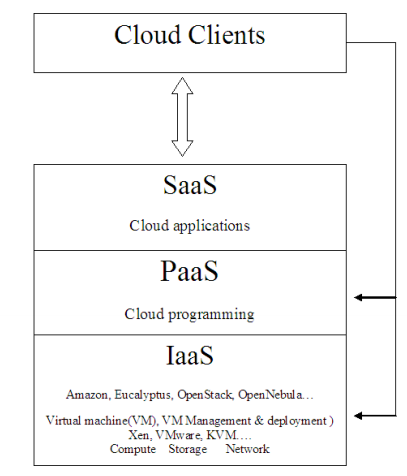
\includegraphics[width=.3\textwidth]{figuras/cloud_structure.png}
\caption{Estrutura de serviços da computação em nuvem. Fonte: \cite{sefraoui2012openstack}}
\label{fig:cloud_structure}
\end{figure}

De acordo com Filho e Dionísio \cite{leite2016influencia} (apud \cite{mell2011nist}), os serviços de nuvens devem possuir as seguintes
características: autoatendimento sob demanda, amplo acesso a rede,
agrupamento de recursos, elasticidade rápida e medição de serviço.

Sefraoui et al. \cite{sefraoui2012openstack} afirmam que a IaaS é onde o recurso de hardware é provido em forma de máquinas vituais. 
O cliente mantém as aplicações, bancos de dados e servidores enquanto o servidor mantém a virtualização da nuvem, 
o hardware, o armazenamento e as redes. 

Para Bhardwaj et al. \cite{bhardwaj2010cloud}, é o serviço de entrega de hardware 
(servidor, armazenamento e rede) e software associado (sistema de arquivos e virtualização de sistemas). Os autores estabelecem
os seguintes serviços a serem providos  por IaaS: Infraestrutura virtual (servidor, armazenamento e rede);
Implantação de aplicativos baseados na Web para fácil disponibilização sob demanda; Balanceamento de carga; 
Estabelecimento de acordos de nível de serviço com os clientes;  Segurança dos CPUs, dados e rede;
e Gestão e provisionamento de conta.

\subsection{Qualidade de Serviço}

A qualidade de serviço na computação em nuvem pode ser considerada como o
desempenho de modo geral do serviço provido \cite{openstack}.

Filho e Dionísio \cite{leite2016influencia} tratam a qualidade de serviço em duas abordagens:
uma relacionada à rede e outra em nível de aplicação. Em relação a rede são tratados
os requisitos para garantir a qualidade do serviço. Em nível de aplicação são tratados
os atributos que implicam no cumprimento dos níveis de serviço acordado. 

A qualidade de serviço também pode ser dividida em dois pontos de vista: o 
ponto de vista do cliente e o ponto de vista do provedor \cite{openstack, bhardwaj2010cloud}. 
O escopo deste trabalho trata apenas das métricas relacionadas ao ponto de vista do provedor.


\section{OpenStack}

O OpenStack é uma ferramenta que fornece serviços de computação em nuvem no modelo IaaS e consiste em um grupo de subprojetos (cada subprojeto é um módulo 
do OpenStack) inter-relacionados 
que controlam um conjunto de recursos de processamento (subprojeto \textit{Nova}), armazenamento (subprojetos \textit{Cinder} e \textit{Swift}),
e de rede (subprojeto \textit{Neutron}) em uma infraestrutura de computação em nuvem \cite{openstack} \cite{bui2016}.

Além desses subprojetos apresentados, o OpenStack conta com alguns serviços compartilhados entre os diferentes módulos, como o serviço de 
autenticação e autorização (subprojeto \textit{Keystone}), serviço de gerenciamento de imagens (subprojeto \textit{Glance}) e o serviço de 
telemetria (subprojeto \textit{Ceilometer}) \cite{openstack}. Estes são apenas os principais serviços providos pelo OpenStack, a
descrição completa de todos os serviços pode ser vista na documentação da ferramenta \cite{openstack}.

O OpenStack é bastante robusto, capaz de controlar uma grande de quantidade
de recursos computacionais em um \textit{data center}, o que exige uma infraestrutura de \textit{hardware} 
considerável para seu funcionamento pleno \cite{openstack_general} \cite{openstack}.

O gerenciamento e controle da infraestrutura da nuvem pelo usuário podem ser realizados por meio de uma aplicação \textit{web}
(subprojeto \textit{Horizon}), via linha de comando (\textit{Command Line Interface} (CLI)) e/ou APIs RESTful \cite{bui2016} \cite{openstack}.
Em relação à integração interna dos módulos do \textit{OpenStack}, esta é realizada por meio de APIs RESTful e 
de \textit{Remote Procedure Call} (RPC) via RabbitMQ (ferramenta que implementa a comunicação inter-processos seguindo o protocolo
\textit{Advanced Message Queue Protocol})\cite{bui2016}. Mais detalhes sobre a integração dos módulos podem ser vistos no estudo de Bui \cite{bui2016}.

A Figura \ref{fig:openstack_architecture} ilustra a arquitetura conceitual do OpenStack, apresentando o relacionamento entre os
módulos que o compõe.

\begin{figure}[ht]
\centering
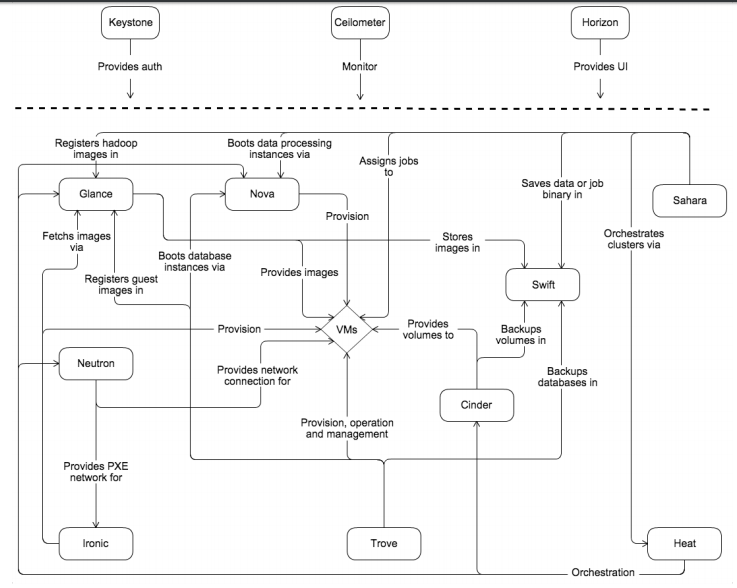
\includegraphics[width=.5\textwidth]{figuras/openstack_architecture.png}
\caption{Arquitetura conceitual do OpenStack. Fonte: \cite{openstack}}
\label{fig:openstack_architecture}
\end{figure}

\section{Materiais e métodos}

Para atingir o objetivo deste trabalho foi utilizada a metodologia apresentada na Figura \ref{metodologia}.

\begin{figure}[ht]
  \centering
  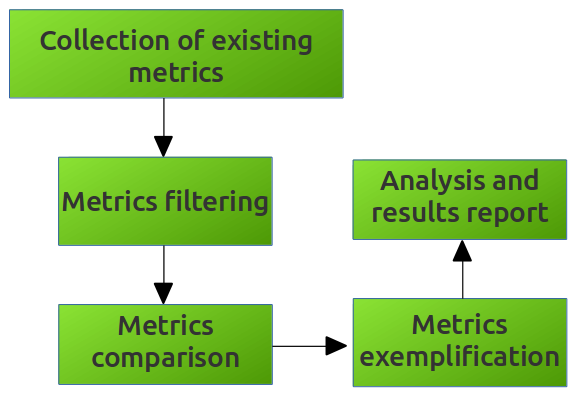
\includegraphics[width=.3\textwidth]{figuras/metodologia.png}
  \caption{Metodologia proposta. Fonte: Autores.}
  \label{metodologia}
\end{figure}


\begin{itemize}
 \item \textbf{Levantamento das métricas existentes} - Esta etapa consistiu em consultar na literatura as métricas de QoS para
	serviços de nuvem e documentá-las, por meio de uma revisão de literatura não sistemática;

 \item \textbf{Filtragem das métricas} - A partir das métricas levantadas com a revisão da literatura, esta etapa consistiu em 
	filtrar os resultados a partir de critérios previamente definidos.
	
 \item \textbf{Confronto das métricas} - Esta etapa consistiu em verificar a existência das métricas filtradas no Openstack,	
	com base na documentação e execução da ferramenta, identificando também como a ferramenta apresenta essa métrica,
	para verificar quais métricas propostas na literatura são implementadas nativamente no OpenStack. Além disso,
	métricas que Openstack fornecia mas não se encontravam na literatura, porém estavam relacionadas com as métricas encontradas,
	foram identificadas e documentadas;
 
 \item \textbf{Validação das métricas} - Esta etapa consistiu em verificar se as métricas confrontadas constavam realmente na ferramenta e
	como eram fornecidas,
	realizando uma simples coleta das métricas idenficadas presentes no Openstack a partir da execução da ferramenta em um cenário de teste.
	Esta etapa englobou as seguintes atividades:
	\subitem - \emph{\textbf{Caracterizar cenário/contexto}}: Nesta atividade descreveu-se o contexto da execução da ferramenta,
		 considerando itens como ambiente para execução do teste, versão da ferramenta utilizada, topologia utilizada, ferramentas
		 e recursos disponíveis;
	\subitem - \emph{\textbf{Elaborar plano de medição}}: Nesta atividade um plano de medição resumido foi criado para guiar a medição
		 a ser feita;
	\subitem - \emph{\textbf{Coletar dados}}: Nesta atividade as métricas foram coletadas e documentadas, seguindo o
		 plano de medição definido anteriormente.

 \item \textbf{Análise e redação dos resultados}: Nesta etapa os resultados obtidos na etapa anterior foram interpretados e documentados.
\end{itemize}

\section{Execução} % MELHORAR ESSE TITULO

  \subsection{Levantamento das métricas existentes}
      
      Foi realizada uma revisão de literatura não sistemática com o intuito de encontrar as métricas de QoS existentes
      propostas em outros estudos. Foram encontrados seis artigos que apresentavam de forma explícita métricas de QoS para
      serviços de nuvem.  Estes artigos foram analisados e foram identificadas 68 métricas que podem ser vistas na Tabela \ref{tab:metricas_literatura}.
      
      \begin{itemize}
       \item \textbf{Artigo 1}: \textit{QoS Metrics for Cloud Computing Services Evaluation} \cite{bardsiri2014};
       \item \textbf{Artigo 2}: \textit{On a Catalogue of Metrics for Evaluating Commercial Cloud Services} \cite{li2012};
       \item \textbf{Artigo 3}: \textit{IaaS Cloud Service Selection using Case-Based Reasoning} \cite{soltani2016};
       \item \textbf{Artigo 4}: \textit{SMICloud: A Framework for Comparing and Ranking Cloud Services} \cite{garg2011};
       \item \textbf{Artigo 5}: \textit{Cloud Services Measures for Global Use} \cite{siegel2012cloud}
       \item \textbf{Artigo 6}: \textit{An End-To-End QoS Mapping Approach for Cloud Service Selection} \cite{karim2013}
      \end{itemize}
      
\begin{table}[]
\centering
 \caption{Métricas encontradas na literatura}
\label{tab:metricas_literatura}
\begin{tabular}{|l|l|l|}
\hline
\multicolumn{1}{|c|}{\textbf{Métrica}}                                                       & \multicolumn{1}{c|}{\textbf{Categoria}}                                                                    & \multicolumn{1}{c|}{\textbf{Artigo}}                                                    \\ \hline
Algoritmos de criptografia                                                                   & Segurança                                                                                                  & \multirow{9}{*}{Artigo 6 [19]}                                                          \\ \cline{1-2}
Apreensibilidade do serviço                                                                  & Usabilidade                                                                                                &                                                                                         \\ \cline{1-2}
Controle de acesso                                                                           & Segurança                                                                                                  &                                                                                         \\ \cline{1-2}
Controle de Dados                                                                            & Controle de Dados                                                                                          &                                                                                         \\ \cline{1-2}
Defeitos por milhão (DPM)                                                                    & -                                                                                                          &                                                                                         \\ \cline{1-2}
Facilidade de uso                                                                            & Usabilidade                                                                                                &                                                                                         \\ \cline{1-2}
Instalabilidade do IaaS                                                                      & Usabilidade                                                                                                &                                                                                         \\ \cline{1-2}
Privacidade dos Dados                                                                        & Segurança                                                                                                  &                                                                                         \\ \cline{1-2}
\begin{tabular}[c]{@{}l@{}}Tempo médio entre \\ falhas (MTBF)\end{tabular}                   & Confiabilidade                                                                                             &                                                                                         \\ \hline
Políticas de controle de acesso                                                              & \begin{tabular}[c]{@{}l@{}}Segurança/ \\ Privacidade\end{tabular}                                          & Artigo 5 [18]                                                                           \\ \hline
Custo de VM                                                                                  & Custo                                                                                                      & \begin{tabular}[c]{@{}l@{}}Artigo 5 [18]; \\ Artigo 4 [1]\end{tabular}                  \\ \hline
\begin{tabular}[c]{@{}l@{}}Armazenamento \\ (memória permanente, ex.HD)\end{tabular}         & -                                                                                                          & \multirow{16}{*}{Artigo 3 [3]}                                                          \\ \cline{1-2}
Banco de dados NoSQL                                                                         & -                                                                                                          &                                                                                         \\ \cline{1-2}
Camadas de aplicação                                                                         & -                                                                                                          &                                                                                         \\ \cline{1-2}
Frequência de CPU                                                                            & -                                                                                                          &                                                                                         \\ \cline{1-2}
Performance de I/O                                                                           & -                                                                                                          &                                                                                         \\ \cline{1-2}
\begin{tabular}[c]{@{}l@{}}Largura de banda \\ (download, upload)\end{tabular}               & -                                                                                                          &                                                                                         \\ \cline{1-2}
Latência máxima (aplicação)                                                                  & -                                                                                                          &                                                                                         \\ \cline{1-2}
Número de balanceadores de carga                                                             & -                                                                                                          &                                                                                         \\ \cline{1-2}
Número de instâncias                                                                         & -                                                                                                          &                                                                                         \\ \cline{1-2}
Número de núcleos de CPU                                                                     & -                                                                                                          &                                                                                         \\ \cline{1-2}
\begin{tabular}[c]{@{}l@{}}Número máximo de \\ usuários concorrentes\end{tabular}            & -                                                                                                          &                                                                                         \\ \cline{1-2}
Região                                                                                       & -                                                                                                          &                                                                                         \\ \cline{1-2}
Servidores de aplicação                                                                      & -                                                                                                          &                                                                                         \\ \cline{1-2}
\begin{tabular}[c]{@{}l@{}}Sistema Operacional\\  (Tipo, Plataforma, Versão)\end{tabular}    & -                                                                                                          &                                                                                         \\ \cline{1-2}
Suporte a SGBD relacional                                                                    & -                                                                                                          &                                                                                         \\ \cline{1-2}
Tipo de aplicação                                                                            & -                                                                                                          &                                                                                         \\ \hline
Segurança (métrica geral)                                                                    & -                                                                                                          & \begin{tabular}[c]{@{}l@{}}Artigo 3 [3]; \\ Artigo 6 [19]\end{tabular}                  \\ \hline
\begin{tabular}[c]{@{}l@{}}Memória (RAM requerida \\ para instância)\end{tabular}            & \begin{tabular}[c]{@{}l@{}}Garantia/ \\ Sustentabilidade \\ do serviço\end{tabular}                        & \multirow{2}{*}{\begin{tabular}[c]{@{}l@{}}Artigo 3 [3]; \\ Artigo 4 [1]\end{tabular}}  \\ \cline{1-2}
Tempo de resposta (aplicação)                                                                & Performance                                                                                                &                                                                                         \\ \hline
Disponibilidade                                                                              & -                                                                                                          & \begin{tabular}[c]{@{}l@{}}Artigo 3 [3]; \\ Artigo 4 [1]; \\ Artigo 6 [19]\end{tabular} \\ \hline
\begin{tabular}[c]{@{}l@{}}Atraso de transferência \\ TCP/UDP/IP\end{tabular}                & \begin{tabular}[c]{@{}l@{}}Performance / \\ Comunicação/ \\ Latência\end{tabular}                          & \multirow{2}{*}{Artigo 2 [4]}                                                           \\ \cline{1-2}
\begin{tabular}[c]{@{}l@{}}Velocidade de transferência \\ bit/byte TCP/UDP/IP\end{tabular}   & \begin{tabular}[c]{@{}l@{}}Performance / \\ Comunicação/ \\ Taxa de transferência \\ de dados\end{tabular} &                                                                                         \\ \hline
Confidencialidade                                                                            & \begin{tabular}[c]{@{}l@{}}Segurança /\\ Autenticação\end{tabular}                                         & \multirow{9}{*}{Artigo 1 [5]}                                                           \\ \cline{1-2}
Efetividade                                                                                  & \begin{tabular}[c]{@{}l@{}}Segurança / \\ Autenticação\end{tabular}                                        &                                                                                         \\ \cline{1-2}
Habilidade de auditoria                                                                      & \begin{tabular}[c]{@{}l@{}}Segurança / \\ Segurança dos dados\end{tabular}                                 &                                                                                         \\ \cline{1-2}
Modularidade                                                                                 & -                                                                                                          &                                                                                         \\ \cline{1-2}
Sensibilidade                                                                                & \begin{tabular}[c]{@{}l@{}}Segurança / \\ Autenticação\end{tabular}                                        &                                                                                         \\ \cline{1-2}
Tempo de boot                                                                                & \begin{tabular}[c]{@{}l@{}}Economia / \\ Elasticidade\end{tabular}                                         &                                                                                         \\ \cline{1-2}
Tempo de computação                                                                          & \begin{tabular}[c]{@{}l@{}}Performance / \\ Tempo\end{tabular}                                             &                                                                                         \\ \cline{1-2}
Utilização de recursos                                                                       & Eficiência                                                                                                 &                                                                                         \\ \cline{1-2}
Velocidade de memória                                                                        & \begin{tabular}[c]{@{}l@{}}Performance /\\  Memória\end{tabular}                                           &                                                                                         \\ \hline
Carga de CPU                                                                                 & \begin{tabular}[c]{@{}l@{}}Performance /\\ Computação\end{tabular}                                         & \multirow{21}{*}{\begin{tabular}[c]{@{}l@{}}Artigo 1 [5]; \\ Artigo 2 [4]\end{tabular}} \\ \cline{1-2}
\begin{tabular}[c]{@{}l@{}}Custo de recursos de \\ componentes\end{tabular}                  & Economia / Custo                                                                                           &                                                                                         \\ \cline{1-2}
Custo por FLOP                                                                               & Economia / Custo                                                                                           &                                                                                         \\ \cline{1-2}
Custo por tempo fixo                                                                         & Economia / Custo                                                                                           &                                                                                         \\ \cline{1-2}
Custo total                                                                                  & Economia / Custo                                                                                           &                                                                                         \\ \cline{1-2}
Eficiência da Instância                                                                      & \begin{tabular}[c]{@{}l@{}}Performance / \\ Computação\end{tabular}                                        &                                                                                         \\ \cline{1-2}
Frequência de perda de pacotes                                                               & \begin{tabular}[c]{@{}l@{}}Performance / \\ Comunicação\end{tabular}                                       &                                                                                         \\ \cline{1-2}
\begin{tabular}[c]{@{}l@{}}Latência de comunicação \\ sobre SSL\end{tabular}                 & \begin{tabular}[c]{@{}l@{}}Segurança / \\ Segurança dos dados\end{tabular}                                 &                                                                                         \\ \cline{1-2}
Razão Preço/Performance                                                                      & Economia / Custo                                                                                           &                                                                                         \\ \cline{1-2}
SSL aplicável?                                                                               & \begin{tabular}[c]{@{}l@{}}Segurança / \\ Segurança dos dados\end{tabular}                                 &                                                                                         \\ \cline{1-2}
Taxa de atualização de RAM                                                                   & \begin{tabular}[c]{@{}l@{}}Performance / \\ Memória\end{tabular}                                           &                                                                                         \\ \cline{1-2}
Taxa de erros de conexão                                                                     & \begin{tabular}[c]{@{}l@{}}Performance / \\ Comunicação\end{tabular}                                       &                                                                                         \\ \cline{1-2}
\begin{tabular}[c]{@{}l@{}}Taxa de FLOPs (Float Point \\ Operations Per Second)\end{tabular} & \begin{tabular}[c]{@{}l@{}}Performance / \\ Computação\end{tabular}                                        &                                                                                         \\ \cline{1-2}
Tempo de comunicação                                                                         & Performance / Tempo                                                                                        &                                                                                         \\ \cline{1-2}
Tempo de deleção                                                                             & \begin{tabular}[c]{@{}l@{}}Economia /\\ Elasticidade\end{tabular}                                          &                                                                                         \\ \cline{1-2}
Tempo de implantação                                                                         & \begin{tabular}[c]{@{}l@{}}Economia / \\ Elasticidade\end{tabular}                                         &                                                                                         \\ \cline{1-2}
Tempo de suspensão                                                                           & \begin{tabular}[c]{@{}l@{}}Economia / \\ Elasticidade\end{tabular}                                         &                                                                                         \\ \cline{1-2}
Tempo total de aquisição                                                                     & \begin{tabular}[c]{@{}l@{}}Economia / \\ Elasticidade\end{tabular}                                         &                                                                                         \\ \cline{1-2}
\begin{tabular}[c]{@{}l@{}}Usuários suportados em um \\ orçamento fixo\end{tabular}          & Economia / Custo                                                                                           &                                                                                         \\ \cline{1-2}
Interoperabilidade                                                                           & -                                                                                                          &                                                                                         \\ \cline{1-2}
Tempo de resposta (memória)                                                                  & \begin{tabular}[c]{@{}l@{}}Performance / \\ Memória\end{tabular}                                           &                                                                                         \\ \hline
Acurácia                                                                                     & -                                                                                                          & \multirow{5}{*}{Artigo 4 [1]}                                                           \\ \cline{1-2}
Adequação                                                                                    & -                                                                                                          &                                                                                         \\ \cline{1-2}
Confiabilidade                                                                               & -                                                                                                          &                                                                                         \\ \cline{1-2}
Elasticidade                                                                                 & -                                                                                                          &                                                                                         \\ \cline{1-2}
Transparência                                                                                & -                                                                                                          &                                                                                         \\ \hline
\end{tabular}
\end{table}

% \begin{table*}[]
% \centering
% \caption{Métricas encontradas na literatura}
% \label{tab:metricas_literatura}
% \begin{tabular}{@{}lccc@{}}
% \toprule
% \multicolumn{1}{c}{\textbf{Métrica}}                                                       & \textbf{Unidade}      & \textbf{Categoria}                                                                                   & \textbf{Artigo}                                                                                  \\ \hline
% Algoritmos de criptografia                                                                   & -                     & Segurança                                                                                            & Artigo 6 {[}19{]}                                                                                \\ \hline
% Apreensibilidade do serviço                                                                  & -                     & Usabilidade                                                                                          & Artigo 6 {[}19{]}                                                                                \\ \hline
% Controle de acesso                                                                           & boolean               & Segurança                                                                                            & Artigo 6 {[}19{]}                                                                                \\ \hline
% Controle de Dados                                                                            & \%                    & Controle de Dados                                                                                    & Artigo 6 {[}19{]}                                                                                \\ \hline
% Defeitos por milhão (DPM)                                                                    & -                     & -                                                                                                    & Artigo 6 {[}19{]}                                                                                \\ \hline
% Facilidade de uso                                                                            & -                     & Usabilidade                                                                                          & Artigo 6 {[}19{]}                                                                                \\ \hline
% Instalabilidade do IaaS                                                                      & -                     & Usabilidade                                                                                          & Artigo 6 {[}19{]}                                                                                \\ \hline
% Privacidade dos Dados                                                                        & -                     & Segurança                                                                                            & Artigo 6 {[}19{]}                                                                                \\ \hline
% Tempo médio entre falhas (MTBF)								     & \%                    & Confiabilidade                                                                                       & Artigo 6 {[}19{]}                                                                                \\ \hline
% Políticas de controle de acesso                                                              & escala ordinal        & Segurança/ Privacidade                                                                               & Artigo 5 {[}18{]}                                                                                \\ \hline
% Custo de VM                                                                                  &                       & Custo;On-going cost base                                                                             & Artigo 5 {[}18{]}; Artigo 4 {[}1{]}                                                              \\ \hline
% \begin{tabular}[c]{@{}l@{}}Armazenamento (memória \\ permanente, ex.HD)\end{tabular}         & GB                    & -                                                                                                    & Artigo 3 {[}3{]}                                                                                 \\ \hline
% Banco de dados NoSQL                                                                         & boolean               & -                                                                                                    & Artigo 3 {[}3{]}                                                                                 \\ \hline
% Camadas de aplicação                                                                         & -                     & -                                                                                                    & Artigo 3 {[}3{]}                                                                                 \\ \hline
% Frequência de CPU                                                                            & MHz, GHz              & -                                                                                                    & Artigo 3 {[}3{]}                                                                                 \\ \hline
% Performance de I/O                                                                           & escala ordinal        & -                                                                                                    & Artigo 3 {[}3{]}                                                                                 \\ \hline
% \begin{tabular}[c]{@{}l@{}}Largura de banda \\ (download, upload)\end{tabular}               & MB/s, GB/s            & -                                                                                                    & Artigo 3 {[}3{]}                                                                                 \\ \hline
% Latência máxima (aplicação)                                                                  & ms                    & -                                                                                                    & Artigo 3 {[}3{]}                                                                                 \\ \hline
% Número de balanceadores de carga                                                             & escala absoluta       & -                                                                                                    & Artigo 3 {[}3{]}                                                                                 \\ \hline
% Número de instâncias                                                                         & escala absoluta       & -                                                                                                    & Artigo 3 {[}3{]}                                                                                 \\ \hline
% Número de núcleos de CPU                                                                     & escala absoluta       & -                                                                                                    & Artigo 3 {[}3{]}                                                                                 \\ \hline
% \begin{tabular}[c]{@{}l@{}}Número máximo de usuários \\ concorrentes\end{tabular}            & escala absoluta       & -                                                                                                    & Artigo 3 {[}3{]}                                                                                 \\ \hline
% Região                                                                                       & -                     & -                                                                                                    & Artigo 3 {[}3{]}                                                                                 \\ \hline
% Servidores de aplicação                                                                      & -                     & -                                                                                                    & Artigo 3 {[}3{]}                                                                                 \\ \hline
% \begin{tabular}[c]{@{}l@{}}Sistema Operacional \\ (Tipo, Plataforma, Versão)\end{tabular}    & escala nominal        & -                                                                                                    & Artigo 3 {[}3{]}                                                                                 \\ \hline
% Suporte a SGBD relacional                                                                    & boolean               & -                                                                                                    & Artigo 3 {[}3{]}                                                                                 \\ \hline
% Tipo de aplicação                                                                            & -                     & -                                                                                                    & Artigo 3 {[}3{]}                                                                                 \\ \hline
% Segurança (métrica geral)                                                                    & escala ordinal; \%    & -                                                                                                    & Artigo 3 {[}3{]}; Artigo 6 {[}19{]}                                                              \\ \hline
% Memória (RAM requerida para instância)                                                       & MB, GB                & Garantia; Sustentabilidade do serviço                                                                & Artigo 3 {[}3{]}; Artigo 4 {[}1{]}                                                               \\ \hline
% Tempo de resposta (aplicação)                                                                & ms                    & Performance                                                                                          & Artigo 3 {[}3{]}; Artigo 4 {[}1{]}                                                               \\ \hline
% Disponibilidade                                                                              & \%                    & -                                                                                                    & \begin{tabular}[c]{@{}c@{}}Artigo 3 {[}3{]}; Artigo 4 {[}1{]}; \\ Artigo 6 {[}19{]}\end{tabular} \\ \hline
% Atraso de transferência TCP/UDP/IP                                                           & s, us                 & Performance / Comunicação/ Latência                                                                  & Artigo 2 {[}4{]}                                                                                 \\ \hline
% \begin{tabular}[c]{@{}l@{}}Velocidade de transferência \\ bit/byte TCP/UDP/IP\end{tabular}   & bps, Mbps, MB/s, GB/s & \begin{tabular}[c]{@{}c@{}}Performance / Comunicação/\\  Taxa de transferência de dados\end{tabular} & Artigo 2 {[}4{]}                                                                                 \\ \hline
% Confidencialidade                                                                            & -                     & Segurança / Autenticação                                                                             & Artigo 1 {[}5{]}                                                                                 \\ \hline
% Efetividade                                                                                  & -                     & Segurança / Autenticação                                                                             & Artigo 1 {[}5{]}                                                                                 \\ \hline
% Habilidade de auditoria                                                                      & boolean               & Segurança / Segurança dos dados                                                                      & Artigo 1 {[}5{]}                                                                                 \\ \hline
% Modularidade                                                                                 & -                     & -                                                                                                    & Artigo 1 {[}5{]}                                                                                 \\ \hline
% Sensibilidade                                                                                & -                     & Segurança / Autenticação                                                                             & Artigo 1 {[}5{]}                                                                                 \\ \hline
% Tempo de boot                                                                                & s                     & Economia / Elasticidade                                                                              & Artigo 1 {[}5{]}                                                                                 \\ \hline
% Tempo de computação                                                                          & -                     & Performance / Tempo                                                                                  & Artigo 1 {[}5{]}                                                                                 \\ \hline
% Utilização de recursos                                                                       & -                     & Eficiência                                                                                           & Artigo 1 {[}5{]}                                                                                 \\ \hline
% Velocidade de memória                                                                        & MB/s, GB/s            & Performance / Memória                                                                                & Artigo 1 {[}5{]}                                                                                 \\ \hline
% Carga de CPU                                                                                 & \%                    & Performance / Computação                                                                             & Artigo 1 {[}5{]}; Artigo 2 {[}4{]}                                                               \\ \hline
% Custo de recursos de componentes                                                             & \$                     & Economia / Custo                                                                                     & Artigo 1 {[}5{]}; Artigo 2 {[}4{]}                                                               \\ \hline
% Custo por FLOP                                                                               & cent/FLOP, \$/GFLOP   & Economia / Custo                                                                                     & Artigo 1 {[}5{]}; Artigo 2 {[}4{]}                                                               \\ \hline
% Custo por tempo fixo                                                                         & \$/ano                & Economia / Custo                                                                                     & Artigo 1 {[}5{]}; Artigo 2 {[}4{]}                                                               \\ \hline
% Custo total                                                                                  & \$                     & Economia / Custo                                                                                     & Artigo 1 {[}5{]}; Artigo 2 {[}4{]}                                                               \\ \hline
% Eficiência da Instância                                                                      & \% de pico de CPU     & Performance / Computação                                                                             & Artigo 1 {[}5{]}; Artigo 2 {[}4{]}                                                               \\ \hline
% Frequência de perda de pacotes                                                               & pacotes/(s, ms)       & Performance / Comunicação                                                                            & Artigo 1 {[}5{]}; Artigo 2 {[}4{]}                                                               \\ \hline
% Latência de comunicação sobre SSL                                                            & ms, s                 & Segurança / Segurança dos dados                                                                      & Artigo 1 {[}5{]}; Artigo 2 {[}4{]}                                                               \\ \hline
% Razão Preço/Performance                                                                      &                       & Economia / Custo                                                                                     & Artigo 1 {[}5{]}; Artigo 2 {[}4{]}                                                               \\ \hline
% SSL aplicável?                                                                               & boolean               & Segurança / Segurança dos dados                                                                      & Artigo 1 {[}5{]}; Artigo 2 {[}4{]}                                                               \\ \hline
% Taxa de atualização de RAM                                                                   & -                     & Performance / Memória                                                                                & Artigo 1 {[}5{]}; Artigo 2 {[}4{]}                                                               \\ \hline
% Taxa de erros de conexão                                                                     & -                     & Performance / Comunicação                                                                            & Artigo 1 {[}5{]}; Artigo 2 {[}4{]}                                                               \\ \hline
% Taxa de FLOPs (Float Point Operations Per Second)                                          & Gflops, TFlops        & Performance / Computação                                                                             & Artigo 1 {[}5{]}; Artigo 2 {[}4{]}                                                               \\ \hline
% Tempo de comunicação                                                                         & s                     & Performance / Tempo                                                                                  & Artigo 1 {[}5{]}; Artigo 2 {[}4{]}                                                               \\ \hline
% Tempo de deleção                                                                             & s                     & Economia / Elasticidade                                                                              & Artigo 1 {[}5{]}; Artigo 2 {[}4{]}                                                               \\ \hline
% Tempo de implantação                                                                         & s                     & Economia / Elasticidade                                                                              & Artigo 1 {[}5{]}; Artigo 2 {[}4{]}                                                               \\ \hline
% Tempo de suspensão                                                                           & s                     & Economia / Elasticidade                                                                              & Artigo 1 {[}5{]}; Artigo 2 {[}4{]}                                                               \\ \hline
% Tempo total de aquisição                                                                     & s                     & Economia / Elasticidade                                                                              & Artigo 1 {[}5{]}; Artigo 2 {[}4{]}                                                               \\ \hline
% \begin{tabular}[c]{@{}l@{}}Usuários suportados em \\ um orçamento fixo\end{tabular}          & usuarios/\$           & Economia / Custo                                                                                     & Artigo 1 {[}5{]}; Artigo 2 {[}4{]}                                                               \\ \hline
% Interoperabilidade                                                                           & -                     & -                                                                                                    & Artigo 1 {[}5{]}; Artigo 4 {[}1{]}                                                               \\ \hline
% Tempo de resposta (memória)                                                                  & ms                    & Performance / Memória                                                                                & Artigo 1 {[}5{]}; Artigo 2 {[}4{]}                                                               \\ \hline
% Acurácia                                                                                     & escala absoluta       & -                                                                                                    & Artigo 4 {[}1{]}                                                                                 \\ \hline
% Adequação                                                                                    & escala ordinal        & -                                                                                                    & Artigo 4 {[}1{]}                                                                                 \\ \hline
% Confiabilidade                                                                               & -                     & -                                                                                                    & Artigo 4 {[}1{]}                                                                                 \\ \hline
% Elasticidade                                                                                 & -                     & -                                                                                                    & Artigo 4 {[}1{]}                                                                                 \\ \hline
% Transparência                                                                                & -                     & -                                                                                                    & Artigo 4 {[}1{]}                                                                                 \\ \hline
% \end{tabular}
% \end{table*}
     
  \subsection{Filtragem das métricas}
  
      Para filtragem das métricas foram definidos quatro critérios considerando o contexto e escopo do trabalho. A avaliação das
      métricas coletadas pode ser vista na Tabela \ref{tab:avaliacao_metricas}.
   
	\begin{itemize}
	 \item \textbf{Critério 1 - O significado é conhecido?}
	    \subitem Esse critério foi utilizado para avaliar se o significado da métrica e sua forma de cálculo, eram conhecidas.
	 \item \textbf{Critério 2 - Aplica-se para o modelo de serviço IaaS?}
	    \subitem Este critério foi utilizado para selecionar as métricas propícias ao modelo IaaS, 
	    devido às suas características peculiares;
% 	    \subitem Este critério foi utilizado pois pode acontecer de algumas métricas se encaixarem mais aos outros modelos
% 		     de serviço e não serem propícias ao modelo IaaS, devido às suas características peculiares;
	 \item \textbf{Critério 3 - Pode ser coletada objetivamente?}
	    \subitem Este critério foi utilizado para selecionar as métricas que são coletadas de forma objetiva, pois esse tipo
	    de métrica pode ser coletado por meio de ferramentas;
	 \item \textbf{Critério 4 - É do ponto de vista do provedor?}
	    \subitem Este critério foi utilizado para selecionar as métricas que se tratavam do ponto de vista do provedor do serviço
	    de nuvem;
	\end{itemize}
	
\begin{table*}[]
\centering
\caption{Avaliação das métricas nos critérios definidos}
\label{tab:avaliacao_metricas}
\begin{tabular}{@{}lcccc@{}}
\toprule
\multicolumn{1}{c}{\textbf{Métrica}}              & \multicolumn{1}{l}{\textbf{Critério 1}} & \multicolumn{1}{l}{\textbf{Critério 2}} & \multicolumn{1}{l}{\textbf{Critério 3}} & \textbf{Critério 4}         \\ \midrule
Atraso de transferência TCP/UDP/IP                & Sim                                     & Sim                                     & Sim                                     & Sim                         \\
Largura de Banda (download, upload)               & Sim                                     & Sim                                     & Sim                                     & Sim                         \\
Carga de CPU                                      & Sim                                     & Sim                                     & Sim                                     & Sim                         \\
Confiabilidade (número de erros)                  & Sim                                     & Sim                                     & Sim                                     & Sim                         \\
Controle de acesso                                & Sim                                     & Sim                                     & Sim                                     & Sim                         \\
Frequência de CPU                                 & Sim                                     & Sim                                     & Sim                                     & Sim                         \\
Custo total                                       & Sim                                     & Sim                                     & Sim                                     & Sim                         \\
Eficiência da Instância                           & Sim                                     & Sim                                     & Sim                                     & Sim                         \\
Elasticidade                                      & Sim                                     & Sim                                     & Sim                                     & Sim                         \\
Frequência de perda de pacotes                    & Sim                                     & Sim                                     & Sim                                     & Sim                         \\
Habilidade de auditoria                           & Sim                                     & Sim                                     & Sim                                     & Sim                         \\
Latência de comunicação sobre SSL                 & Sim                                     & Sim                                     & Sim                                     & Sim                         \\
Latência máxima (aplicação)                       & Sim                                     & Sim                                     & Sim                                     & Sim                         \\
Número máximo de usuários concorrentes            & Sim                                     & Sim                                     & Sim                                     & Sim                         \\
Memória (RAM requerida para instância)            & Sim                                     & Sim                                     & Sim                                     & Sim                         \\
Suporte a banco de dados NoSQL                    & Sim                                     & Sim                                     & Sim                                     & Sim                         \\
Número de núcleos de CPU                          & Sim                                     & Sim                                     & Sim                                     & Sim                         \\
Número de instância                               & Sim                                     & Sim                                     & Sim                                     & Sim                         \\
Número de balanceadores de carga                  & Sim                                     & Sim                                     & Sim                                     & Sim                         \\
Sistema Operacional (Tipo, Plataforma, Versão)    & Sim                                     & Sim                                     & Sim                                     & Sim                         \\
Suporte a SGBD relacional                         & Sim                                     & Sim                                     & Sim                                     & Sim                         \\
Tempo de resposta (memória)                       & Sim                                     & Sim                                     & Sim                                     & Sim                         \\
SSL aplicável?                                    & Sim                                     & Sim                                     & Sim                                     & Sim                         \\
Armazenamento (Memória permanente. ex: HD)        & Sim                                     & Sim                                     & Sim                                     & Sim                         \\
Tempo de boot                                     & Sim                                     & Sim                                     & Sim                                     & Sim                         \\
Tempo de comunicação                              & Sim                                     & Sim                                     & Sim                                     & Sim                         \\
Tempo de deleção                                  & Sim                                     & Sim                                     & Sim                                     & Sim                         \\
Tempo de implantação                              & Sim                                     & Sim                                     & Sim                                     & Sim                         \\
Tempo de resposta (aplicação)                     & Sim                                     & Sim                                     & Sim                                     & Sim                         \\
Tempo de suspensão                                & Sim                                     & Sim                                     & Sim                                     & Sim                         \\
Tempo médio entre falhas (MTBF)                   & Sim                                     & Sim                                     & Sim                                     & Sim                         \\
Tempo total de aquisição                          & Sim                                     & Sim                                     & Sim                                     & Sim                         \\
Velocidade de transferência bit/byte TCP/UDP/IP   & Sim                                     & Sim                                     & Sim                                     & Sim                         \\
Performance de I/O                                & Sim                                     & Sim                                     & Sim                                     & Sim                         \\
Acurácia                                          & Sim                                     & Sim                                     & Sim                                     & \cellcolor[HTML]{EA9999}Não \\
Disponibilidade                                   & Sim                                     & Sim                                     & Sim                                     & \cellcolor[HTML]{EA9999}Não \\
Adequação                                         & Sim                                     & \cellcolor[HTML]{EA9999}Não             & \cellcolor[HTML]{EA9999}-               & \cellcolor[HTML]{EA9999}-   \\
Apreensibilidade do serviço                       & Sim                                     & Sim                                     & \cellcolor[HTML]{EA9999}Não             & \cellcolor[HTML]{EA9999}-   \\
Controle de Dados                                 & Sim                                     & Sim                                     & \cellcolor[HTML]{EA9999}Não             & \cellcolor[HTML]{EA9999}-   \\
Custo por tempo fixo                              & Sim                                     & Sim                                     & \cellcolor[HTML]{EA9999}Não             & \cellcolor[HTML]{EA9999}-   \\
Defeitos por milhão                               & Sim                                     & \cellcolor[HTML]{EA9999}Não             & \cellcolor[HTML]{EA9999}-               & \cellcolor[HTML]{EA9999}-   \\
Facilidade de uso                                 & Sim                                     & Sim                                     & \cellcolor[HTML]{EA9999}Não             & \cellcolor[HTML]{EA9999}-   \\
Instalabilidade do IaaS                           & Sim                                     & Sim                                     & \cellcolor[HTML]{EA9999}Não             & \cellcolor[HTML]{EA9999}-   \\
Interoperabilidade                                & Sim                                     & Sim                                     & \cellcolor[HTML]{EA9999}Não             & \cellcolor[HTML]{EA9999}-   \\
Políticas de controle de acesso                   & Sim                                     & Sim                                     & \cellcolor[HTML]{EA9999}Não             & \cellcolor[HTML]{EA9999}-   \\
Transparência                                     & Sim                                     & Sim                                     & \cellcolor[HTML]{EA9999}Não             & \cellcolor[HTML]{EA9999}-   \\
Custo de VM                                       & Sim                                     & Sim                                     & \cellcolor[HTML]{EA9999}Não             & \cellcolor[HTML]{EA9999}-   \\
Algoritmos de criptografia                        & \cellcolor[HTML]{EA9999}Não             & \cellcolor[HTML]{EA9999}-               & \cellcolor[HTML]{EA9999}-               & \cellcolor[HTML]{EA9999}-   \\
Servidores de aplicação                           & \cellcolor[HTML]{EA9999}Não             & \cellcolor[HTML]{EA9999}-               & \cellcolor[HTML]{EA9999}-               & \cellcolor[HTML]{EA9999}-   \\
Camadas de aplicação                              & \cellcolor[HTML]{EA9999}Não             & \cellcolor[HTML]{EA9999}-               & \cellcolor[HTML]{EA9999}-               & \cellcolor[HTML]{EA9999}-   \\
Tipo de aplicação                                 & \cellcolor[HTML]{EA9999}Não             & \cellcolor[HTML]{EA9999}-               & \cellcolor[HTML]{EA9999}-               & \cellcolor[HTML]{EA9999}-   \\
Confidencialidade                                 & \cellcolor[HTML]{EA9999}Não             & \cellcolor[HTML]{EA9999}-               & \cellcolor[HTML]{EA9999}-               & \cellcolor[HTML]{EA9999}-   \\
Custo de recursos de componentes                  & \cellcolor[HTML]{EA9999}Não             & \cellcolor[HTML]{EA9999}-               & \cellcolor[HTML]{EA9999}-               & \cellcolor[HTML]{EA9999}-   \\
Custo por FLOP                                    & \cellcolor[HTML]{EA9999}Não             & \cellcolor[HTML]{EA9999}-               & \cellcolor[HTML]{EA9999}-               & \cellcolor[HTML]{EA9999}-   \\
Efetividade                                       & \cellcolor[HTML]{EA9999}Não             & \cellcolor[HTML]{EA9999}-               & \cellcolor[HTML]{EA9999}-               & \cellcolor[HTML]{EA9999}-   \\
Modularidade                                      & \cellcolor[HTML]{EA9999}Não             & \cellcolor[HTML]{EA9999}-               & \cellcolor[HTML]{EA9999}-               & \cellcolor[HTML]{EA9999}-   \\
Privacidade dos Dados                             & \cellcolor[HTML]{EA9999}Não             & \cellcolor[HTML]{EA9999}-               & \cellcolor[HTML]{EA9999}-               & \cellcolor[HTML]{EA9999}-   \\
Razão Preço/Performance                           & \cellcolor[HTML]{EA9999}Não             & \cellcolor[HTML]{EA9999}-               & \cellcolor[HTML]{EA9999}-               & \cellcolor[HTML]{EA9999}-   \\
Região                                            & \cellcolor[HTML]{EA9999}Não             & \cellcolor[HTML]{EA9999}-               & \cellcolor[HTML]{EA9999}-               & \cellcolor[HTML]{EA9999}-   \\
Segurança (métrica geral)                         & \cellcolor[HTML]{EA9999}Não             & \cellcolor[HTML]{EA9999}-               & \cellcolor[HTML]{EA9999}-               & \cellcolor[HTML]{EA9999}-   \\
Sensibilidade                                     & \cellcolor[HTML]{EA9999}Não             & \cellcolor[HTML]{EA9999}-               & \cellcolor[HTML]{EA9999}-               & \cellcolor[HTML]{EA9999}-   \\
Taxa de atualização de RAM                        & \cellcolor[HTML]{EA9999}Não             & \cellcolor[HTML]{EA9999}-               & \cellcolor[HTML]{EA9999}-               & \cellcolor[HTML]{EA9999}-   \\
Taxa de FLOPs (Float Point Operations Per Second) & \cellcolor[HTML]{EA9999}Não             & \cellcolor[HTML]{EA9999}-               & \cellcolor[HTML]{EA9999}-               & \cellcolor[HTML]{EA9999}-   \\
Tempo de computação                               & \cellcolor[HTML]{EA9999}Não             & \cellcolor[HTML]{EA9999}-               & \cellcolor[HTML]{EA9999}-               & \cellcolor[HTML]{EA9999}-   \\
Usuários suportados em um orçamento fixo          & \cellcolor[HTML]{EA9999}Não             & \cellcolor[HTML]{EA9999}-               & \cellcolor[HTML]{EA9999}-               & \cellcolor[HTML]{EA9999}-   \\
Utilização de recursos                            & \cellcolor[HTML]{EA9999}Não             & \cellcolor[HTML]{EA9999}-               & \cellcolor[HTML]{EA9999}-               & \cellcolor[HTML]{EA9999}-   \\
Velocidade de memória                             & \cellcolor[HTML]{EA9999}Não             & \cellcolor[HTML]{EA9999}-               & \cellcolor[HTML]{EA9999}-               & \cellcolor[HTML]{EA9999}-   \\
Taxa de erros de conexão                          & \cellcolor[HTML]{EA9999}Não             & \cellcolor[HTML]{EA9999}-               & \cellcolor[HTML]{EA9999}-               & \cellcolor[HTML]{EA9999}-   \\ \bottomrule
\end{tabular}
\end{table*}
   
  \subsection{Confronto das métricas} \label{confronto}
  
  Com a filtragem obteve-se 34 métricas resultantes a serem confrontadas no Openstack. Para isso, as métricas foram divididas em estáticas e
  dinâmicas, ou seja, aquelas que não necessitam de execução da ferramenta para serem coletadas e aquelas que necessitam da execução da ferramenta,
  respectivamente. Além disso, as métricas foram categorizadas com base no estudo de Bardsiri e Hashemi \cite{bardsiri2014}.As categorias foram:
  Confiabilidade, Economia, Memória, Performance, Segurança e Geral. Vale ressaltar, que foram identificadas duas métricas equivalentes (Velocidade de transferência bit/byte TCP/UDP/IP
  e Largura de Banda (download, upload)) e dessa forma, apenas a Largura de Banda foi considerada na avaliação.
  
  A categorização e o confronto das métricas pode ser visualizado nas Tabelas   \ref{tab:confronto_estaticas} e \ref{tab:confronto_dinamicas}  
 que representam as métricas estáticas e dinâmicas, respectivamente. 

\begin{table}[ht]
\centering
\caption{Avaliação das métricas estáticas existentes no Openstack}
\label{tab:confronto_estaticas}
\begin{tabular}{@{}lll@{}}
\toprule
\multicolumn{3}{c}{\textbf{Estáticas}}                                                                  \\ \midrule
\textbf{Categoria}         & \textbf{Métrica}                               & \textbf{Há no Openstack?} \\
Economia                   & Custo total                                    & -                         \\
\multirow{3}{*}{Geral}     & Suporte a banco de dados NoSQL                 & Sim                       \\
                           & \begin{tabular}[c]{@{}l@{}}Sistema Operacional \\ (Tipo, Plataforma, Versão)\end{tabular} & Sim                       \\
                           & Suporte a SGBD relacional                      & Sim                       \\
\multirow{3}{*}{Segurança} & Controle de acesso                             & Sim                       \\
                           & SSL aplicável?                                 & Sim                       \\
                           & Habilidade de auditoria                        & Sim                       \\ \bottomrule
\end{tabular}
\end{table}  

\begin{table}[ht]
\centering
\caption{Avaliação das métricas dinâmicas existentes no Openstack}
\label{tab:confronto_dinamicas}
\begin{tabular}{@{}lll@{}}
\toprule
\multicolumn{1}{c}{Dinâmicas}          &                                                                                       &                                               \\ \midrule
\multicolumn{1}{c}{\textbf{Categoria}} & \multicolumn{1}{c}{\textbf{Métrica}}                                                  & \multicolumn{1}{c}{\textbf{Há no Openstack?}} \\
\multirow{2}{*}{Confiabilidade}        & Confiabilidade (número de erros)                                                      & Não                                           \\
                                       & Tempo médio entre falhas (MTBF)                                                       & Não                                           \\
\multirow{6}{*}{Economia}              & Elasticidade                                                                          & Não                                           \\
                                       & Tempo de boot                                                                         & Não                                           \\
                                       & Tempo de deleção                                                                      & Não                                           \\
                                       & Tempo de implantação                                                                  & Não                                           \\
                                       & Tempo de suspensão                                                                    & Não                                           \\
                                       & Tempo total de aquisição                                                              & Não                                           \\
\multirow{2}{*}{Memória}               & \begin{tabular}[c]{@{}l@{}}Memória (RAM requerida \\ para instância)\end{tabular}     & Sim                                           \\
                                       & \begin{tabular}[c]{@{}l@{}}Armazenamento (Memória \\ permanente. ex: HD)\end{tabular} & Sim                                           \\
\multirow{15}{*}{Performance}          & Latência máxima  (aplicação)                                                          & Não                                           \\
                                       & \begin{tabular}[c]{@{}l@{}}Número máximo de usuários \\ concorrentes\end{tabular}     & Não                                           \\
                                       & Número de núcleos de CPU                                                              & Não                                           \\
                                       & Número de instâncias                                                                  & Sim                                           \\
                                       & Número de balanceadores de carga                                                      & Não                                           \\
                                       & Tempo de resposta (aplicação)                                                         & Não                                           \\
                                       & Largura de Banda (download, upload)                                                   & Sim                                           \\
                                       & Carga de CPU                                                                          & Sim                                           \\
                                       & Frequência de CPU                                                                     & Sim                                           \\
                                       & Eficiência da Instância                                                               & Sim                                           \\
                                       & Frequência de perda de pacotes                                                        & Não                                           \\
                                       & Atraso de transferência TCP/UDP/IP                                                    & Não                                           \\
                                       & Performance de I/O                                                                    & Sim                                           \\
                                       & Tempo de resposta (memória)                                                           & Não                                           \\
                                       & Tempo de comunicação                                                                  & Não                                           \\
Segurança                              & Latência de comunicação sobre SSL                                                     & Não                                           \\ \bottomrule
\end{tabular}
\end{table}  

As métricas existentes no Openstack podem ser sumarizadas nos itens abaixo.
Além das métricas idênticas ao que foi levantado, foram identificadas outras
métricas relacionadas. Todas as métricas fornecidas pela ferramenta podem ser consultadas na documentação \cite{openstack}.

\begin{itemize}
 \item \textbf{Memória (RAM requerida para instância)}
    \subitem - Volume de RAM alocado para a instância (memory);
    \subitem - Volume de RAM utilizado pela instância (memory.usage);
    \subitem - Volume de RAM utilizada por projeto.
 \item \textbf{Armazenamento (Memória permanente. ex: HD)}
    \subitem - Tamanho do disco do nó de processamento (disk.root.size);
    \subitem - Memória permanente utilizada por projeto;
    \subitem - Memória permante utilizada por instância.
 \item \textbf{Latência máxima  (aplicação)}
    \subitem - Latência média do disco (disk.latency);
    \subitem - Latência média do disco por dispositivo (disk.device.latency).
 \item \textbf{Número de núcleos de CPU}
    \subitem - Número de CPUs virtuais alocadas para a instância (vcpus);
    \subitem - Número de CPUs virtuais por projeto;
    \subitem - Média de utilização de CPU (cpu\_util).
 \item \textbf{Número de instâncias}
    \subitem - Número de instâncias ativas.
 \item \textbf{Número de balanceadores de carga}
    \subitem - Existência de um pool de balanceador de carga (network.services.lb.pool);
    \subitem - Existência de um balanceador de carga VIP (network.services.lb.vip);
    \subitem - Existência de um membro de balanceador de carga (network.services.lb.member);
    \subitem - Existência de um balanceador de carga health probe (network.services.lb.health\_monitor);
    \subitem - Total de conexões em um balanceador de carga (network.services.lb.total.connections);
    \subitem - Conexões ativas em um balanceador de carga (network.services.lb.active.connections).
  \item \textbf{Largura de Banda (download, upload)}
    \subitem - Bytes via roteadores de rótulo L3 (roteadores de camada de rede) (bandwidth).
  \item \textbf{Carga de CPU}   
    \subitem - Carga de CPU no último 1 minuto (hardware.cpu.load.1min);
    \subitem - Carga de CPU nos últimos 5 minutos (hardware.cpu.load.5min);
    \subitem - Carga de CPU nos últimos 10 minutos (hardware.cpu.load.10min);
  \item \textbf{Frequência de CPU}  
    \subitem - Frequência da CPU (compute.node.cpu.frequency);
  \item \textbf{Eficiência da Instância}    
    \subitem - Utilização da CPU (compute.node.cpu.percent);
    \item \textbf{Frequência de perda de pacotes}   
    \subitem - Taxa de entrada de pacotes (network.incoming.packets.rate);
    \subitem - Taxa de saída de pacotes (network.outgoing.packets.rate);
  \item \textbf{Performance de I/O} 
    \subitem - Número de requisições de leitura (disk.read.requests);
    \subitem - Taxa média de requisições de leitura (disk.read.requests.rate);
    \subitem - Número de requisições de escrita (disk.write.requests);
    \subitem - Taxa média de requisições de escrita (disk.write.requests.rate);
    \subitem - Volume de leitura (disk.read.bytes);
    \subitem - Taxa média de leituras (disk.read.bytes.rate);
    \subitem - Volume de escritas (disk.write.bytes);
    \subitem - Taxa média de escritas (disk.write.bytes.rate);
 \end{itemize}  

  \subsection{Validação das métricas} 
    Para verificar como se apresentavam as métricas ditas presentes no OpenStack, foi executado um cenário de teste de uso da ferramenta
    para coletar tais métricas obtidas na seção \ref{confronto}. 
    A Subseção \ref{cenario} descreve o cenário utilizado, a Subseção \ref{plano_medicao} apresenta o planejamento para a
    coleta dos dados realizado e a Subseção \ref{resultados_levantamento} discorre sobre os resultados obtidos.
  
    \subsubsection{\textbf{Cenário de teste}} \label{cenario}
	
	A coleta dos dados foi realizada no seguinte cenário/contexto:
	
	\begin{itemize}
	 \item Duas pessoas com dedicação parcial como equipe de coleta; % COLOCA DEDICAÇÃO PARCIAL ?
	 \item Laboratório com máquinas que possuiam recursos de \textit{hardware} simples;
	    \subitem Apenas máquinas com 4GB de memória RAM no máximo.
	 \item Utilização da versão \textit{Kilo} do OpenStack;
	 \item Utilização do CentOS 7 \cite{centos} como sistema operacional;
	 \item Utilização da topologia apresentada na Figura \ref{fig:topologia};
	    \subitem Foram utilizados dois computadores interconectados para distribuir a carga de processamento entre eles, 
		     de modo que um computador ficava com o nó Controlador (\textit{Controller}) e o outro computador ficava
		     com os nós de Processamento (\textit{Compute}) e de Rede (\textit{Network}), como ilustra a Figura \ref{fig:topologia}.
	    \subitem A topologia utilizada foi baseada na topologia proposta por Ahmad Imanudin em \cite{imanudin}.
	\end{itemize}
	 
	\begin{figure}[ht]
	\centering
	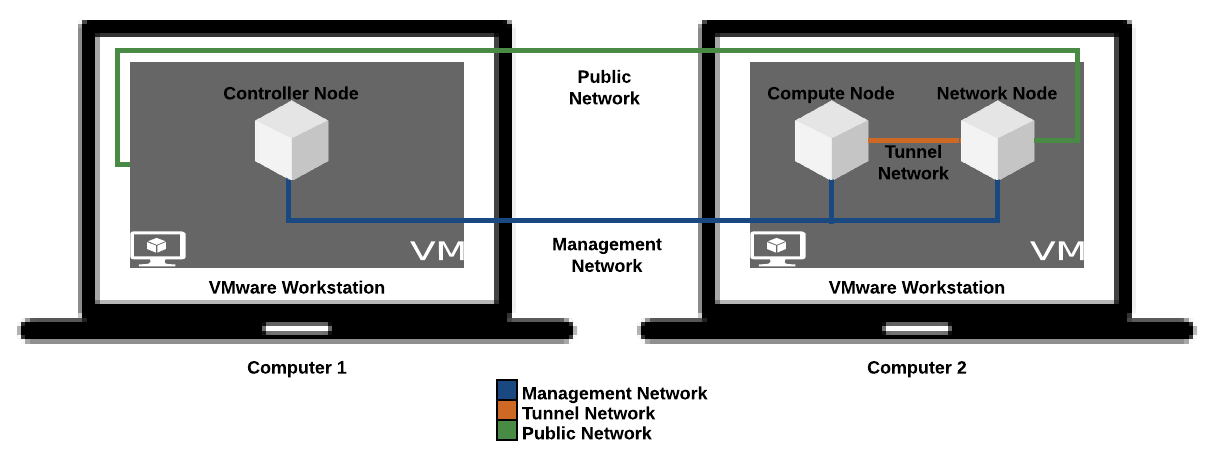
\includegraphics[width=.5\textwidth]{figuras/topologia.png}
	\caption{Topologia utilizada no cenário de teste. Fonte: Autor.}
	\label{fig:topologia}
	\end{figure}
	
	Foi utilizada a versão \textit{Kilo} \cite{openstack_kilo} do OpenStack por ser uma versão estável e mais leve, devido a
	limitação dos recursos disponíveis.
	Vale ressaltar que apesar do suporte para versão \textit{Kilo} ter sido encerrado pelos mantenedores do OpenStack,
	sua arquitetura não distoa muito do seu sucessor subsequente ainda suportado, o OpenStack \textit{Liberty}, o que
	não impacta significativamente nem invalida o presente trabalho \cite{openstack_liberty}.

	
	%%%%%%%%%%%%%%%%%%%%%%%%%%%%%%
% % % %  PROBLEMA: O OpenStack Kilo já está em End-Of-Life... Versão ainda suportada: Liberty.
% % % %  Ou colocar como trabalho futuro, ou tentar trocar a versão.
	%%%%%%%%%%%%%%%%%%%%%%%%%%%%%%
    
%     \subsubsection{Plano de Medição} \label{plano_medicao}
%     
%     \subsubsection{Resultados} \label{resultados_levantamento}
  

\section{Conclusão}
Com a revisão de literatura realizada foi possível coletar 68 métricas relacionadas a QoS para serviços de nuvem, das quais
35 foram avaliadas no Openstack. Na avaliação foi possível perceber que o Openstack provia 40\% das métricas exatas e além disso
possuia algumas outras métricas relacionadas com as métricas identificadas.

% .....

Uma limitação identificada do trabalho é que foi considerada uma versão antiga da ferramenta. Outra limitação é que as métricas
foram identificadas por uma revisão simples de literatura, o que não possibilitou uma visibilidade do máximo de trabalhos possíveis,
ou seja, foram considerados poucos estudos relacionados.

Como proposta de trabalho futuro é vista a aplicação de uma revisão sistemática com o intuito de encontrar mais métricas e aplicá-las para
uma versão mais atual do Openstack.


%%%%%%%%%%%%%%%%%%%%%%%%%%%%%%%%%

% % Propor os requisitos de hardware (RAM, HD) como métrica de QoS

%%%%%%%%%%%%%%%%%%%%%%%%%%%%%%%%%


% \subsection{Subsection Heading Here}
% Subsection text here.
% 
% 
% \subsubsection{Subsubsection Heading Here}
% Subsubsection text here.


% An example of a floating figure using the graphicx package.
% Note that \label must occur AFTER (or within) \caption.
% For figures, \caption should occur after the \includegraphics.
% Note that IEEEtran v1.7 and later has special internal code that
% is designed to preserve the operation of \label within \caption
% even when the captionsoff option is in effect. However, because
% of issues like this, it may be the safest practice to put all your
% \label just after \caption rather than within \caption{}.
%
% Reminder: the "draftcls" or "draftclsnofoot", not "draft", class
% option should be used if it is desired that the figures are to be
% displayed while in draft mode.
%
%\begin{figure}[!t]
%\centering
%\includegraphics[width=2.5in]{myfigure}
% where an .eps filename suffix will be assumed under latex, 
% and a .pdf suffix will be assumed for pdflatex; or what has been declared
% via \DeclareGraphicsExtensions.
%\caption{Simulation results for the network.}
%\label{fig_sim}
%\end{figure}

% Note that the IEEE typically puts floats only at the top, even when this
% results in a large percentage of a column being occupied by floats.


% An example of a double column floating figure using two subfigures.
% (The subfig.sty package must be loaded for this to work.)
% The subfigure \label commands are set within each subfloat command,
% and the \label for the overall figure must come after \caption.
% \hfil is used as a separator to get equal spacing.
% Watch out that the combined width of all the subfigures on a 
% line do not exceed the text width or a line break will occur.
%
% \begin{figure*}[!t]
% \centering
% \subfloat[Case I]{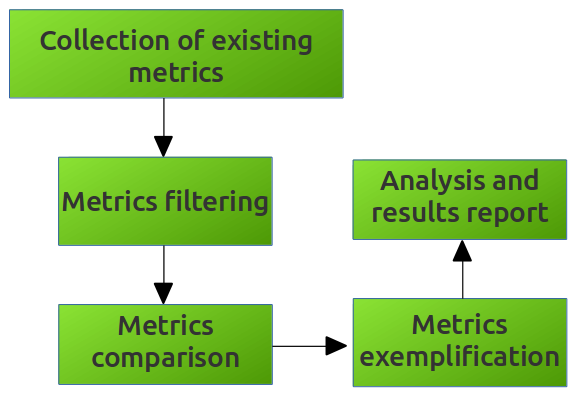
\includegraphics[width=2.5in]{figuras/metodologia}%
% \label{fig_first_case}}
% \hfil
% \subfloat[Case II]{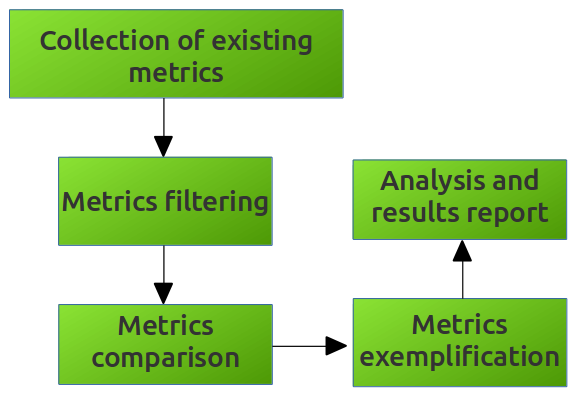
\includegraphics[width=2.5in]{figuras/metodologia}%
% \label{fig_second_case}}
% \caption{Simulation results for the network.}
% \label{fig_sim}
% \end{figure*}
%
% Note that often IEEE papers with subfigures do not employ subfigure
% captions (using the optional argument to \subfloat[]), but instead will
% reference/describe all of them (a), (b), etc., within the main caption.
% Be aware that for subfig.sty to generate the (a), (b), etc., subfigure
% labels, the optional argument to \subfloat must be present. If a
% subcaption is not desired, just leave its contents blank,
% e.g., \subfloat[].


% An example of a floating table. Note that, for IEEE style tables, the
% \caption command should come BEFORE the table and, given that table
% captions serve much like titles, are usually capitalized except for words
% such as a, an, and, as, at, but, by, for, in, nor, of, on, or, the, to
% and up, which are usually not capitalized unless they are the first or
% last word of the caption. Table text will default to \footnotesize as
% the IEEE normally uses this smaller font for tables.
% The \label must come after \caption as always.
%
%\begin{table}[!t]
%% increase table row spacing, adjust to taste
%\renewcommand{\arraystretch}{1.3}
% if using array.sty, it might be a good idea to tweak the value of
% \extrarowheight as needed to properly center the text within the cells
%\caption{An Example of a Table}
%\label{table_example}
%\centering
%% Some packages, such as MDW tools, offer better commands for making tables
%% than the plain LaTeX2e tabular which is used here.
%\begin{tabular}{|c||c|}
%\hline
%One & Two\\
%\hline
%Three & Four\\
%\hline
%\end{tabular}
%\end{table}


% Note that the IEEE does not put floats in the very first column
% - or typically anywhere on the first page for that matter. Also,
% in-text middle ("here") positioning is typically not used, but it
% is allowed and encouraged for Computer Society conferences (but
% not Computer Society journals). Most IEEE journals/conferences use
% top floats exclusively. 
% Note that, LaTeX2e, unlike IEEE journals/conferences, places
% footnotes above bottom floats. This can be corrected via the
% \fnbelowfloat command of the stfloats package.

% conference papers do not normally have an appendix


% use section* for acknowledgment
% \section*{Acknowledgment}


% The authors would like to thank...





% trigger a \newpage just before the given reference
% number - used to balance the columns on the last page
% adjust value as needed - may need to be readjusted if
% the document is modified later
%\IEEEtriggeratref{8}
% The "triggered" command can be changed if desired:
%\IEEEtriggercmd{\enlargethispage{-5in}}

% references section

% can use a bibliography generated by BibTeX as a .bbl file
% BibTeX documentation can be easily obtained at:
% http://mirror.ctan.org/biblio/bibtex/contrib/doc/
% The IEEEtran BibTeX style support page is at:
% http://www.michaelshell.org/tex/ieeetran/bibtex/
%\bibliographystyle{IEEEtran}
% argument is your BibTeX string definitions and bibliography database(s)
%\bibliography{IEEEabrv,../bib/paper}
%
% <OR> manually copy in the resultant .bbl file
% set second argument of \begin to the number of references
% (used to reserve space for the reference number labels box)

% Please add the following required packages to your document preamble:
% \usepackage{multirow}

\bibliographystyle{IEEEtran}
\bibliography{references}
% \begin{thebibliography}{1}
% 
% \bibitem{IEEEhowto:kopka}
% H.~Kopka and P.~W. Daly, \emph{A Guide to \LaTeX}, 3rd~ed.\hskip 1em plus
%   0.5em minus 0.4em\relax Harlow, England: Addison-Wesley, 1999.
% 
% \end{thebibliography}




% that's all folks
\end{document}


